% questions.tex —— 2006 年·上海卷·文科 · 题目内容片段（无答案）
% 由 tools/generate_projects.py 依来源总账自 2006/2006_数学真题_上海文_试题.md 生成，勿手改（改源 MD 后重跑）


\gkpart{数学}

\begin{gktip}
\raggedright
\textbf{来源说明}：题面按固定 PDF 印刷页码 330–331 转录。该 PDF 与第三方 GitHub 镜像 \texttt{deekur/gaokaomath} 固定提交 \texttt{34c13a6cf632c0b69c95f89b9b923bbc4a08924d} 路径 \texttt{普通高考/2006/2006上海文.pdf} 的 Git blob（\texttt{82b54c4337468a5a1182d4bbef76831a0de98f33}）逐字节一致；SHA-256 为 \texttt{1881e13e917febc73882254c59200be192286802042d650c82956f8901c2d174}。上海市教育考试院归档页《2006年秋季高考上海卷数学(文史)试题及答案》用于确认考试身份并核对官方答案，但不证明该镜像 PDF 是官方原件。扫描件原出版者、版次和数字化来源链仍未知；固定 PDF 共两页 A3 题面，不附答案页。

\textbf{图形说明}：第 12、13、18、19 题按固定题面可见信息重绘为本卷 \texttt{figures/} 下的 TikZ 矢量源；未将原卷截图作为图形资产入库。
\end{gktip}

\gkpart{一、填空题}

\begin{question}
\gkti{1}已知集合 $A=\{-1,3,m\}$，集合 $B=\{3,4\}$。若 $B\subseteq A$，则实数 $m=$ \gkblank{}。

\end{question}
\begin{question}
\gkti{2}已知两条直线 $l_1:ax+3y-3=0$，$l_2:4x+6y-1=0$。若 $l_1\parallel l_2$，则 $a=$ \gkblank{}。

\end{question}
\begin{question}
\gkti{3}若函数 $f(x)=a^x$（$a>0$，且 $a\ne1$）的反函数的图象过点 $(2,-1)$，则 $a=$ \gkblank{}。

\end{question}
\begin{question}
\gkti{4}计算：$\displaystyle\lim_{n\to\infty}\frac{n(n^2+1)}{6n^3+1}=$ \gkblank{}。

\end{question}
\begin{question}
\gkti{5}若复数 $z=(m-2)+(m+1)i$ 为纯虚数（$i$ 为虚数单位），其中 $m\in\mathbb R$，则 $|z|=$ \gkblank{}。

\end{question}
\begin{question}
\gkti{6}函数 $y=\sin x\cos x$ 的最小正周期是 \gkblank{}。

\end{question}
\begin{question}
\gkti{7}已知双曲线的中心在原点，一个顶点的坐标是 $(3,0)$，且焦距与虚轴长之比为 $5:4$，则双曲线的标准方程是 \gkblank{}。

\end{question}
\begin{question}
\gkti{8}方程 $\log_3(x^2-10)=1+\log_3x$ 的解是 \gkblank{}。

\end{question}
\begin{question}
\gkti{9}已知实数 $x,y$ 满足
\nopagebreak[4]
\[
\begin{cases}
x+y-3\geqslant0,\\
x+2y-5\leqslant0,\\
x\geqslant0,\\
y\geqslant0,
\end{cases}
\]
则 $y-2x$ 的最大值是 \gkblank{}。

\end{question}
\begin{question}
\gkti{10}在一个小组中有 8 名女同学和 4 名男同学，从中任意地挑选 2 名同学担任交通安全宣传志愿者，那么选到的两名都是女同学的概率是 \gkblank{}。（结果用分数表示）

\end{question}
\begin{question}
\gkti{11}若曲线 $|y|=2^x+1$ 与直线 $y=b$ 没有公共点，则 $b$ 的取值范围是 \gkblank{}。

\Needspace{0.4\textheight}
\end{question}
\begin{question}
\gkti{12}如图，平面中两条直线 $l_1$ 和 $l_2$ 相交于点 $O$。对于平面上任意一点 $M$，若 $p,q$ 分别是 $M$ 到直线 $l_1,l_2$ 的距离，则称有序非负实数对 $(p,q)$ 是点 $M$ 的“距离坐标”。根据上述定义，“距离坐标”是 $(1,2)$ 的点的个数是 \gkblank{}。
\nopagebreak[4]
\begin{center}% 2006 上海卷文科 Q12；按固定扫描件印刷页 330 的可见拓扑绘制。
\begin{tikzpicture}[line cap=round,line join=round]
  \coordinate (O) at (0,0);
  \coordinate (P) at (1.55,1.55);
  \coordinate (M) at (2.25,0.85);
  \coordinate (Q) at (2.25,0);

  \draw[thick] (-1.8,-1.8)--(3.1,3.1);
  \node[above] at (2.75,2.75) {$l_1$};
  \draw[thick] (-1.9,0)--(2.75,0);
  \node[left] at (-1.9,0) {$l_2$};

  \draw[dashed] (M)--(P);
  \draw[dashed] (M)--(Q);
  % 两个直角小方框均按原图绘制，不为垂足添加原图没有的标签。
  \draw[thin] (P)--++(-0.14,-0.14)--++(0.14,-0.14)--++(0.14,0.14);
  \draw[thin] (Q)--++(-0.14,0)--++(0,0.14)--++(0.14,0);

  \node[below right=1pt] at (O) {$O$};
  \fill (M) circle[radius=1.2pt];
  \node[right] at (M) {$M(p,q)$};
\end{tikzpicture}
\end{center}
\nopagebreak[4]
\end{question}
\gkpart{二、选择题}

\Needspace{0.4\textheight}
\begin{question}
\gkti{13}如图，在平行四边形 $ABCD$ 中，下列结论中错误的是\mbox{（　　）}

（A）$\overrightarrow{AB}=\overrightarrow{DC}$　（B）$\overrightarrow{AD}+\overrightarrow{AB}=\overrightarrow{AC}$

（C）$\overrightarrow{AB}-\overrightarrow{AD}=\overrightarrow{BD}$　（D）$\overrightarrow{AD}+\overrightarrow{CB}=\vec 0$
\nopagebreak[4]
\begin{center}% 2006 上海卷文科 Q13；只保留原图中的平行四边形轮廓与四个顶点标签。
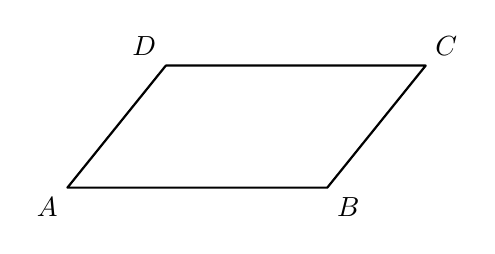
\begin{tikzpicture}[line cap=round,line join=round]
  \coordinate (A) at (0,0);
  \coordinate (B) at (3.3,0);
  \coordinate (C) at (4.55,1.55);
  \coordinate (D) at (1.25,1.55);

  \draw[thick] (A)--(B)--(C)--(D)--(A);
  \node[below left] at (A) {$A$};
  \node[below right] at (B) {$B$};
  \node[above right] at (C) {$C$};
  \node[above left] at (D) {$D$};
\end{tikzpicture}
\end{center}
\nopagebreak[4]
\end{question}
\begin{question}
\gkti{14}如果 $a<0,b>0$，那么下列不等式中正确的是\mbox{（　　）}

\begin{gkopts}(2)
\task （A）$\dfrac1a<\dfrac1b$
\task （B）$\sqrt{-a}<\sqrt b$
\task （C）$a^2<b^2$
\task （D）$|a|>|b|$
\end{gkopts}

\end{question}
\begin{question}
\gkti{15}若空间中有两条直线，则“这两条直线为异面直线”是“这两条直线没有公共点”的\mbox{（　　）}

（A）充分非必要条件　（B）必要非充分条件\\
（C）充分必要条件　（D）既非充分又非必要条件

\end{question}
\begin{question}
\gkti{16}如果一条直线与一个平面垂直，那么，称此直线与平面构成一个“正交线面对”。在一个正方体中，由两个顶点确定的直线与含有四个顶点的平面构成的“正交线面对”的个数是\mbox{（　　）}

\begin{gkopts}(4)
\task （A）48
\task （B）18
\task （C）24
\task （D）36
\end{gkopts}

\end{question}
\gkpart{三、解答题}

\begin{question}
\gkti{17}已知 $\alpha$ 是第一象限的角，且 $\cos\alpha=\dfrac5{13}$，求 $\displaystyle\frac{\sin\left(\alpha+\frac\pi4\right)}{\cos(2\alpha+4\pi)}$ 的值。

\Needspace{0.4\textheight}
\end{question}
\begin{question}
\gkti{18}如图，当甲船位于 $A$ 处时获悉，在其正东方向相距 20 海里的 $B$ 处有一艘渔船遇险等待营救。甲船立即前往救援，同时把消息告知在甲船的南偏西 $30^\circ$、相距 10 海里 $C$ 处的乙船，试问乙船应朝北偏东多少度的方向沿直线前往 $B$ 处救援？（角度精确到 $1^\circ$）
\nopagebreak[4]
\begin{center}% 2006 上海卷文科 Q18；线段长度和方向按题面与来源图标注，示意图不按比例。
\begin{tikzpicture}[line cap=round,line join=round]
  \coordinate (A) at (0,0);
  \coordinate (B) at (4.3,0);
  \coordinate (C) at (-1.5,-2.598);

  % 原图中位于 A 左侧及穿过 A 的两条方位参考虚线。
  \draw[dashed] (-1.45,0)--(A);
  \draw[dashed] (0,1.75)--(0,-1.45);
  \draw[->] (0.72,1.05)--(0.72,2.05);
  \node[above] at (0.72,2.05) {北};

  \draw[thick] (A)--(B);
  \draw[thick] (A)--(C);
  \draw (0,-0.66) arc[start angle=-90,end angle=-120,radius=0.66];
  \node[above] at (2.15,0) {$20$};
  \node[left] at (-0.92,-1.42) {$10$};
  \node at (-0.28,-0.92) {$30^\circ$};

  \fill (A) circle[radius=1.2pt];
  \fill (B) circle[radius=1.2pt];
  \fill (C) circle[radius=1.2pt];
  \node[above left] at (A) {$A$};
  \node[above right] at (B) {$B$};
  \node[below left] at (C) {$C$};
\end{tikzpicture}
\end{center}
\nopagebreak[4]
\Needspace{0.4\textheight}
\end{question}
\begin{question}
\gkti{19}在直三棱柱 $ABC-A_1B_1C_1$ 中，$\angle ABC=90^\circ$，$AB=BC=1$。

（1） 求异面直线 $B_1C_1$ 与 $AC$ 所成角的大小；

（2） 若 $A_1C$ 与平面 $ABC$ 所成角为 $45^\circ$，求三棱锥 $A_1-ABC$ 的体积。
\nopagebreak[4]
\begin{center}% 2006 上海卷文科 Q19；按固定扫描件印刷页 330 重绘，线型与连接关系为核对重点。
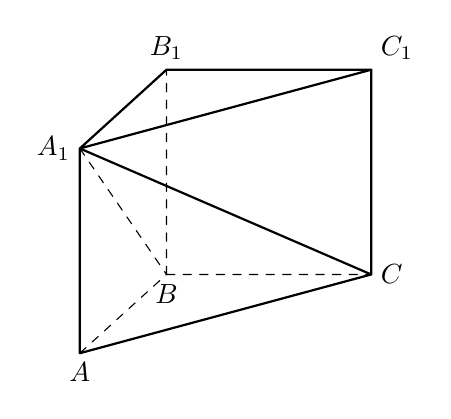
\begin{tikzpicture}[line cap=round,line join=round]
  \coordinate (A)  at (0,0);
  \coordinate (B)  at (1.1,1.0);
  \coordinate (C)  at (3.7,1.0);
  \coordinate (A1) at (0,2.6);
  \coordinate (B1) at (1.1,3.6);
  \coordinate (C1) at (3.7,3.6);

  % 来源图中的隐藏棱以及 A_1B 辅助线为虚线。
  \draw[dashed] (A)--(B) (B)--(C) (B)--(B1) (A1)--(B);
  \draw[thick] (A)--(A1) (C)--(C1) (A)--(C);
  \draw[thick] (A1)--(B1) (B1)--(C1) (A1)--(C1);
  \draw[thick] (A1)--(C);

  \node[below] at (A) {$A$};
  \node[below] at (B) {$B$};
  \node[right] at (C) {$C$};
  \node[left] at (A1) {$A_1$};
  \node[above] at (B1) {$B_1$};
  \node[above right] at (C1) {$C_1$};
\end{tikzpicture}
\end{center}
\nopagebreak[4]
\end{question}
\begin{question}
\gkti{20}设数列 $\{a_n\}$ 的前 $n$ 项和为 $S_n$，且对任意正整数 $n$，$a_n+S_n=4096$。

（1） 求数列 $\{a_n\}$ 的通项公式；

（2） 设数列 $\{\log_2a_n\}$ 的前 $n$ 项和为 $T_n$，对数列 $\{T_n\}$，从第几项起 $T_n<-509$？

\end{question}
\begin{question}
\gkti{21}已知在平面直角坐标系 $xOy$ 中的一个椭圆，它的中心在原点，左焦点为 $F(-\sqrt3,0)$，且右顶点为 $D(2,0)$，设点 $A$ 的坐标是 $\left(1,\dfrac12\right)$。

（1） 求该椭圆的标准方程；

（2） 若 $P$ 是椭圆上的动点，求线段 $PA$ 中点 $M$ 的轨迹方程；

（3） 过原点 $O$ 的直线交椭圆于点 $B,C$，求 $\triangle ABC$ 面积的最大值。

\end{question}
\begin{question}
\gkti{22}已知函数 $y=x+\dfrac ax$ 有如下性质：如果常数 $a>0$，那么该函数在 $(0,\sqrt a]$ 上是减函数，在 $[\sqrt a,+\infty)$ 上是增函数。

（1） 如果函数 $y=x+\dfrac{2^b}{x}$（$x>0$）在 $(0,4]$ 上是减函数，在 $[4,+\infty)$ 上是增函数，求 $b$ 的值；

（2） 设常数 $c\in[1,4]$，求函数 $f(x)=x+\dfrac cx$（$1\leqslant x\leqslant2$）的最大值和最小值；

（3） 当 $n$ 是正整数时，研究函数 $g(x)=x^n+\dfrac c{x^n}$（$c>0$）的单调性，并说明理由。

\end{question}